
\documentclass[a4paper,11pt]{article}
%   Document Standards
    \usepackage[utf8]{inputenc}
    \usepackage[T1]{fontenc}
    \usepackage{lmodern}
    
    \usepackage{dsfont}
	\usepackage{mathtools}

% German language support
	 \usepackage[ngerman,british]{babel}

%   Mathematics
	\usepackage[pdftex]{graphicx}
	\usepackage{latexsym}
    \usepackage{amsmath}
    \usepackage{amssymb}
    \usepackage{amsthm}
    \usepackage{amsfonts}
    \usepackage{mathrsfs}
    \usepackage{listings}
\usepackage{caption}
\usepackage{subcaption}
\usepackage{float}
\usepackage{wrapfig}
\usepackage{extarrows}
\usepackage{thmtools,thm-restate}

    
    \usepackage[dvipsnames]{xcolor}
	\usepackage{framed}
	\colorlet{shadecolor}{gray!12}

%   Formatting
    \usepackage{graphicx}   % Graphics
    \usepackage{booktabs}   % Tables
    \usepackage{fancyhdr}   % Headers and footers
    \usepackage{caption}
    %\usepackage{subcaption}
   	\usepackage[left]{eurosym}
    \usepackage{enumerate}
    \usepackage{tabularx}
    \usepackage{array}
    \usepackage{xcolor}
    \usepackage{rotating}
    \usepackage{multirow}
    \usepackage{natbib}
	\usepackage{apalike}
    \usepackage{pdflscape} % gedrehte Seiten
    \usepackage{wrapfig} % textumflossene Tabellen
    \usepackage{url}
    \usepackage{multicol}
    
	\usepackage{todonotes}    
    \usepackage{multirow}
    \usepackage{booktabs} 
    \usepackage{longtable}
    
    \usepackage{tikz}
	\usetikzlibrary{calc}    
    \usepackage{float}
    
\newsavebox{\tablebox} 
\definecolor{gray3}{gray}{0.3}

\usepackage[a4paper, left=3cm, right=3cm, top=4cm, textheight=23cm]{geometry}	
				
\usepackage{hyperref}
				
%\setlength{\parindent}{0pt}
				
%define colours



\title{Test Title}
\author{}
\setlength{\parindent}{0pt}


\begin{document}
% \maketitle

\begin{abstract}
We build a model that predicts a wine's quality based on its chemical properties. We use a Bayesian linear regression as a model and can thus determine the posterior probability of a wine being of outstanding quality. Applying this model out of sample will show us that vodka might be the best wine of them all \dots or maybe the model should only be applied to Portuguese red wines.
\end{abstract}

\section{Introduction}

We want to predict the quality and taste of a red wine without time and cost intensive surveys. Instead we want to use the chemical attributes of a wine to predict its quality on a scale from 1 to 10.
We are particularly interested in the probability that the wine scores at least a 7/10 as these exclusive wines might distributed through different channels with a more tailored pricing.

\section{Data}
We use a \underline{\href{https://archive.ics.uci.edu/ml/datasets/wine+quality}{\color{blue}wine dataset}} made available by \cite{wine-data}. It contains the chemical properties and quality of 1599 Portuguese wines. The data has the following columns:
\begin{multicols}{3}
\begin{enumerate}
\item fixed acidity 
\item volatile acidity 
\item citric acid 
\item residual sugar 
\item chlorides 
\item free sulfur dioxide 
\item total sulfur dioxide 
\item density 
\item pH 
\item sulphates 
\item alcohol 
\item quality
\end{enumerate}
\end{multicols}

This data obviously fits the problem we are trying to answer. The data is already well cleaned and has no missing values or obvious errors.

The data was also graphically analysed. As an example Figure \ref{fig:corr} shows the correlation between the different columns of the red wine dataset. We can see that most variables have only a week linear correlation with the wine's quality. The quality is most strongly correlated with the alcohol content and the volatile acidity.

\begin{figure}[H]
\centering
	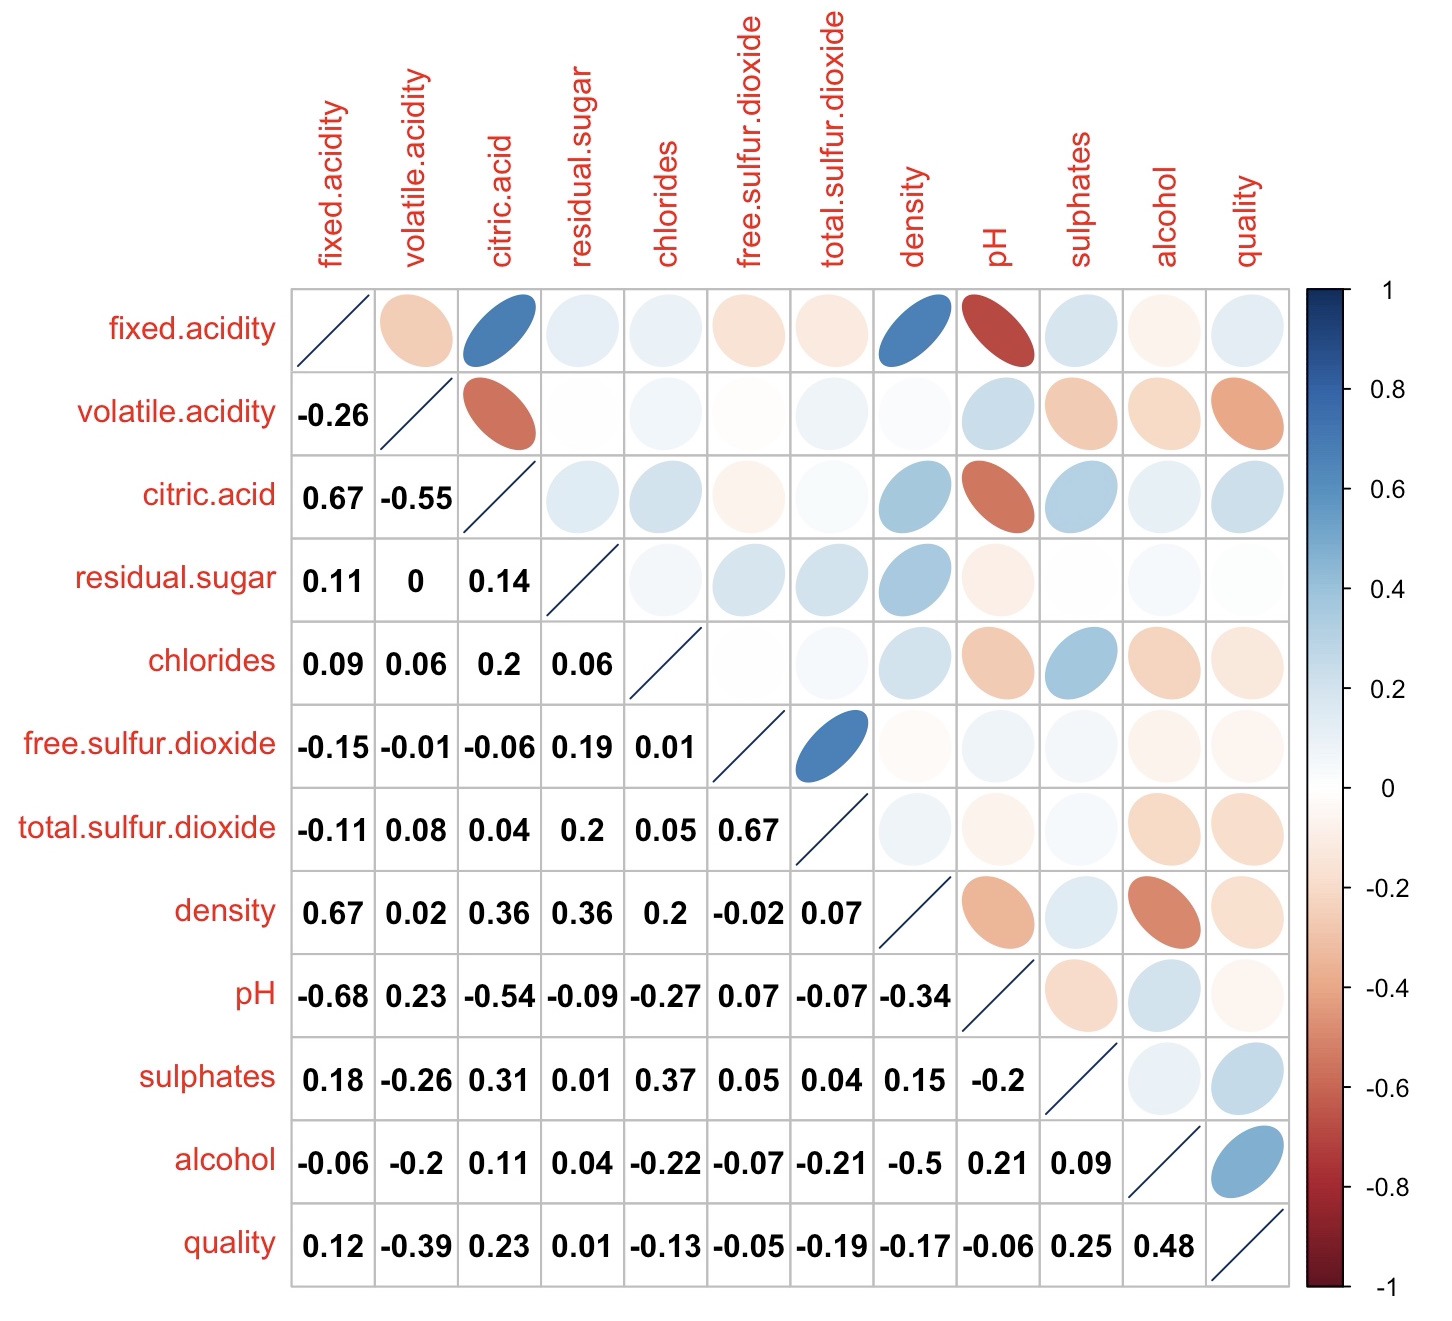
\includegraphics[width=0.4\textwidth]{corr.jpeg}
	\caption{Correlation plot of the data}
	\label{fig:corr}
\end{figure}


\section{Model}

To predict the quality scores of different wines a regression model is needed and a linear model seems a good first guess. The quality score, albeit being discrete, can be thought of as taking continuous values and the rounded value is given in the dataset. So, we postulate the following Bayesian linear regression model
\begin{align}
\begin{split}
y_i |\ \mu_i, \sigma &\stackrel{\text{ind.}}{\sim} N(\mu_i, \sigma^2),\\
\mu_i &= \beta_0 + X \beta,
\end{split}
\end{align}
where $X$ is the data matrix and $\beta$ the vector of regression coefficients. To decide which of the parameters are relevant we use a non-informative prior, which allows us to use the R implementation of the linear model. We use the AIC to decide which parameters to keep. This results in the following parameters:
\begin{multicols}{3}
\begin{enumerate}
\item volatile acidity 
\item chlorides 
\item free sulfur dioxide 
\item total sulfur dioxide 
\item pH 
\item sulphates 
\item alcohol 
\end{enumerate}
\end{multicols}

This leads to the following model
\begin{align}
\begin{split}
y_i |\ \mu_i, \sigma &\stackrel{\text{ind.}}{\sim} N(\mu_i, \sigma^2),\\
\mu_i &= \beta_0 + \beta_1x_{1,i} + \beta_2x_{2,i} + \beta_3x_{3,i}  + \beta_4x_{4,i}  + \beta_1x_{4,i}  + \beta_5x_{5,i}  + \beta_6x_{6,i} + \beta_7x_{7,i},\\
\beta_i &\stackrel{\text{iid.}}{\sim} N(0, 10^6), \ i =0,\dots, 7 \\
\sigma^2 & \sim IG(0.5, 0.5)
\end{split}
\end{align}
The priors are chosen in a way to obtain little information as, we have no prior conception of what the values should be.
The model was fitted in R. As the diagnostics and plots showed a strong autocorrelation for some variables, we chose to iterate the MC chain for 500,000 steps and keep every 50th value. after taking these measures the trace plots and diagnostics looked fine.

The model assumptions seems to be met as the Q-Q plot, see Figure \ref{fig:qq}, indicates that residuals are approximately normally distributed and show a standard deviation of 0.64, which indicates a good fit, particularly considering that the \emph{true values} we compare the model to are rounded to the nearest integer.

\begin{figure}[H]
\centering
	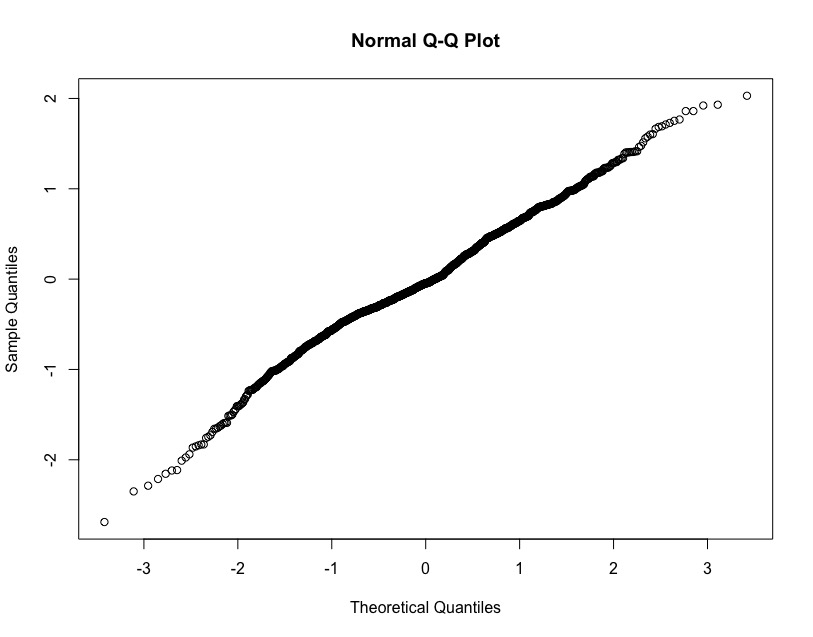
\includegraphics[width=0.4\textwidth]{qqplot.jpeg}
	\caption{Q-Q plot of the residuals}
	\label{fig:qq}
\end{figure}

We fitted a second linear model with only volatile acidity and alcohol, the two variables most strongly correlated with the quality, as explanatory variables. However, the DIC is higher than for the model described above, indicating a less adequate model.

\section{Results}
Looking at the posterior distributions, we see that all coefficient are significantly different from zero. We also see that the posterior probability that alcohol has a positive influence on the wine quality is basically 1.
We want to predict the score of a wine with a feature vector of $(0.35, 0.073, 18, 38, 3.4, 0.87, 13.6)$. The mean posterior quality is 6.95 and the posterior probability that the wine is exceptional (score $\geq 7$) is 17\%. 

However, one needs to be careful to use the model only for data similar to the given dataset as the mean posterior quality score for vodka (feature vector $(0, 0.01, 0, 0, 6, 0, 40)$) is an astonishing 13/10.

\section{Conclusion}
We learnt that in the 21st century humans do not need to bother themselves with deciding what wine they like when computers can do that more efficiently. Though it might come as a surprise to many when a vodka wins the best wine of the year award.

\bibliographystyle{apalike}
\bibliography{Bib.bib}

\end{document}